\subsection{Architecture hybride \og orientée états\fg{}}
\label{sec:comm_state}

Les premiers travaux liés à cette thèse \cite{Desprat2015a,Desprat2015b} se sont 
intéressés principalement à la mise en place de l'architecture de communication 
en basant les structures de données sur des états (plutôt que des événements). 
Cette section décrit les choix fait lors de la modélisation de l'architecture \og 
orientée état\fg{}, pour le stockage et le transfert par exemple, en lien fort avec les 
technologies web sous-jacentes.  
%l'architecture est principalement s'app
%The client-server part is based on a REST (Representa- tional State Transfer) 
%architecture [TV10] that benefits from distributed hypermedia systems such as 
%our. 
%
%
%Pros
%Easier to maintain
%No need to keep a permanent an open connection
%Web context: use of HTTP protocol, URI as resource representative, server 
%caching
%
%
%Cons
%Bandwidth increasing and latency: client needs to keep locally all the necessary 
%data to send the request
%  Table 1 resumes the advantages and the drawbacks of a RESTful system. It 
%fits 
%  well for web distributed sys- tems even if mobile devices should have limited 
%  perfor- mance due to back and forth requests that are energy consuming.
%  
\subsubsection{Spécificité des composants de l'architecture}
Le système présenté repose sur une architecture \acrshort{REST} 
(\acrlong{REST}) concernant les échanges clients-serveur. Cette architecture 
permet de séparer les responsabilités entre le client et le serveur en séparant 
l'\gls{IU} du stockage. \gls{REST} propose une interface uniforme. Cela implique 
que chaque ressource est identifiée et manipulable par des représentation définies 
(modification, suppression). 

Chaque pair correspond a un client (navigateur web) qui contient l'intergiciel 
\gls{P2P} offrant des fonctionnalités limitées, l'interface utilisateur contenant 
l'environnement \gls{3D} et un espace de stockage reposant local (IndexedDB).

La persistance long terme est une base de données NoSQL. Ce type de base de 
données a tendance à être optimisée en lecture (grâce à un 
langage de requête dédié) et permet d'éviter les 
structures rigides. Cette flexibilité est utile lors du stockage des modèles \gls{3D} 
et 
encourage la conservation d'autres méta données (ex: relations entre les différents 
objets) pour faciliter la traçabilité. 
Avec une base de données centralisée, le système possède une source de 
données fiable et autoritaire qui permet à un utilisateur de récupérer le bon contenu 
quand il revient sur une scène. La totalité du document contenant la scène est 
envoyé à l'utilisateur lorsqu'il y accède.


\subsubsection{Gestion du stockage et structure de données}

Avec une base de données NoSQL utilisant des schémas dynamiques, les 
données sont stockées sous forme de document. Chaque document est 
auto-descriptif et peut contenir des valeurs qui s'imbriquent sous la forme d'une 
structure en arbre hiérarchique. Une collection consiste à grouper des documents, 
équivalent dnas une base de données relationnelle à la notion de table. La base de 
données contient deux types de collections : les scènes et les géométries. Une 
collection de scènes contient des scènes qui sont décrites par leur identifiant et 
les méta-données de l'espace virtuel \gls{3D} ainsi que la liste des contributeurs et 
la 
liste des maillages. Cette liste correspond à une association entre un identifiant de 
maillage, les méta-données de l'objet et l'identifiant d'une géométrie existante. 
Les géométries sont, quant à elles, stockées avec leur identifiant propre et l'objet 
3D complet donné sous le format \gls{JSON}.

Localement, sur chaque client, il existe un stockage relationnel (IndexedDB) pour 
chaque objet de la base de donnée récupérée. Cela permet au client de faire des 
requêtes directement dans son espace local si besoin d'ajouter un maillage par 
exemple. 
C'est également une source pour transférer ses modifications aux autres clients.
Les navigateurs permettent désormais de stocker de quantités de données 
importante localement avec une durée de vie illimitée. 
Les paramètres des opérations fondamentales sur la base de données 
(\gls{CRUD}) sur les collections sont très bien supportés par les requêtes 
\gls{REST}.


\subsubsection{Gestion de la session}
Lorsqu'un utilisateur rejoint une session, il suit le déroulement des opérations 
décrit dans la Figure \ref{fig:sequence_state}. 
Dans un premier temps, afin de récupérer les données liées à l'espace de travail, 
le client web de l'utilisateur qui se rend sur une scène récupère 
tous les objets associés à la scène dans la base de données. Les objets de la 
scènes sont renvoyés à l'éditeur pour les afficher. 
Dans un second temps, le système établit les connexions \gls{P2P} entre les 
clients de manière automatique et complète (topologie réseau en maillage 
complet) après avoir récupéré les identifiants des autres utilisateurs auprès du 
serveur de \textit{signaling}. Une fois la connexion établie, chaque collaborateur 
voit son environnement \gls{3D} dans l'éditeur mis à jour, indiquant la position du 
nouvel 
arrivant. Les collaborateurs éditent ensuite la scène \gls{3D} qui produit, sur les 
différents objets, des requêtes \gls{CRUD} -- incluant les opérations de translation, 
rotation et homothétie -- destinées au serveur (qui transmet les 
modifications à la base de données) puis aux collaborateurs.
Enfin, dans un dernier temps, lorsque l'utilisateur quitte la scène, il en notifie le 
serveur de \textit{signaling} qui s'occupe d'indiquer aux clients restants, l'abandon 
du client pour qu'ils puissent mettre à jour leur interface en conséquence.

\begin{figure}[ht!]
	\centering
	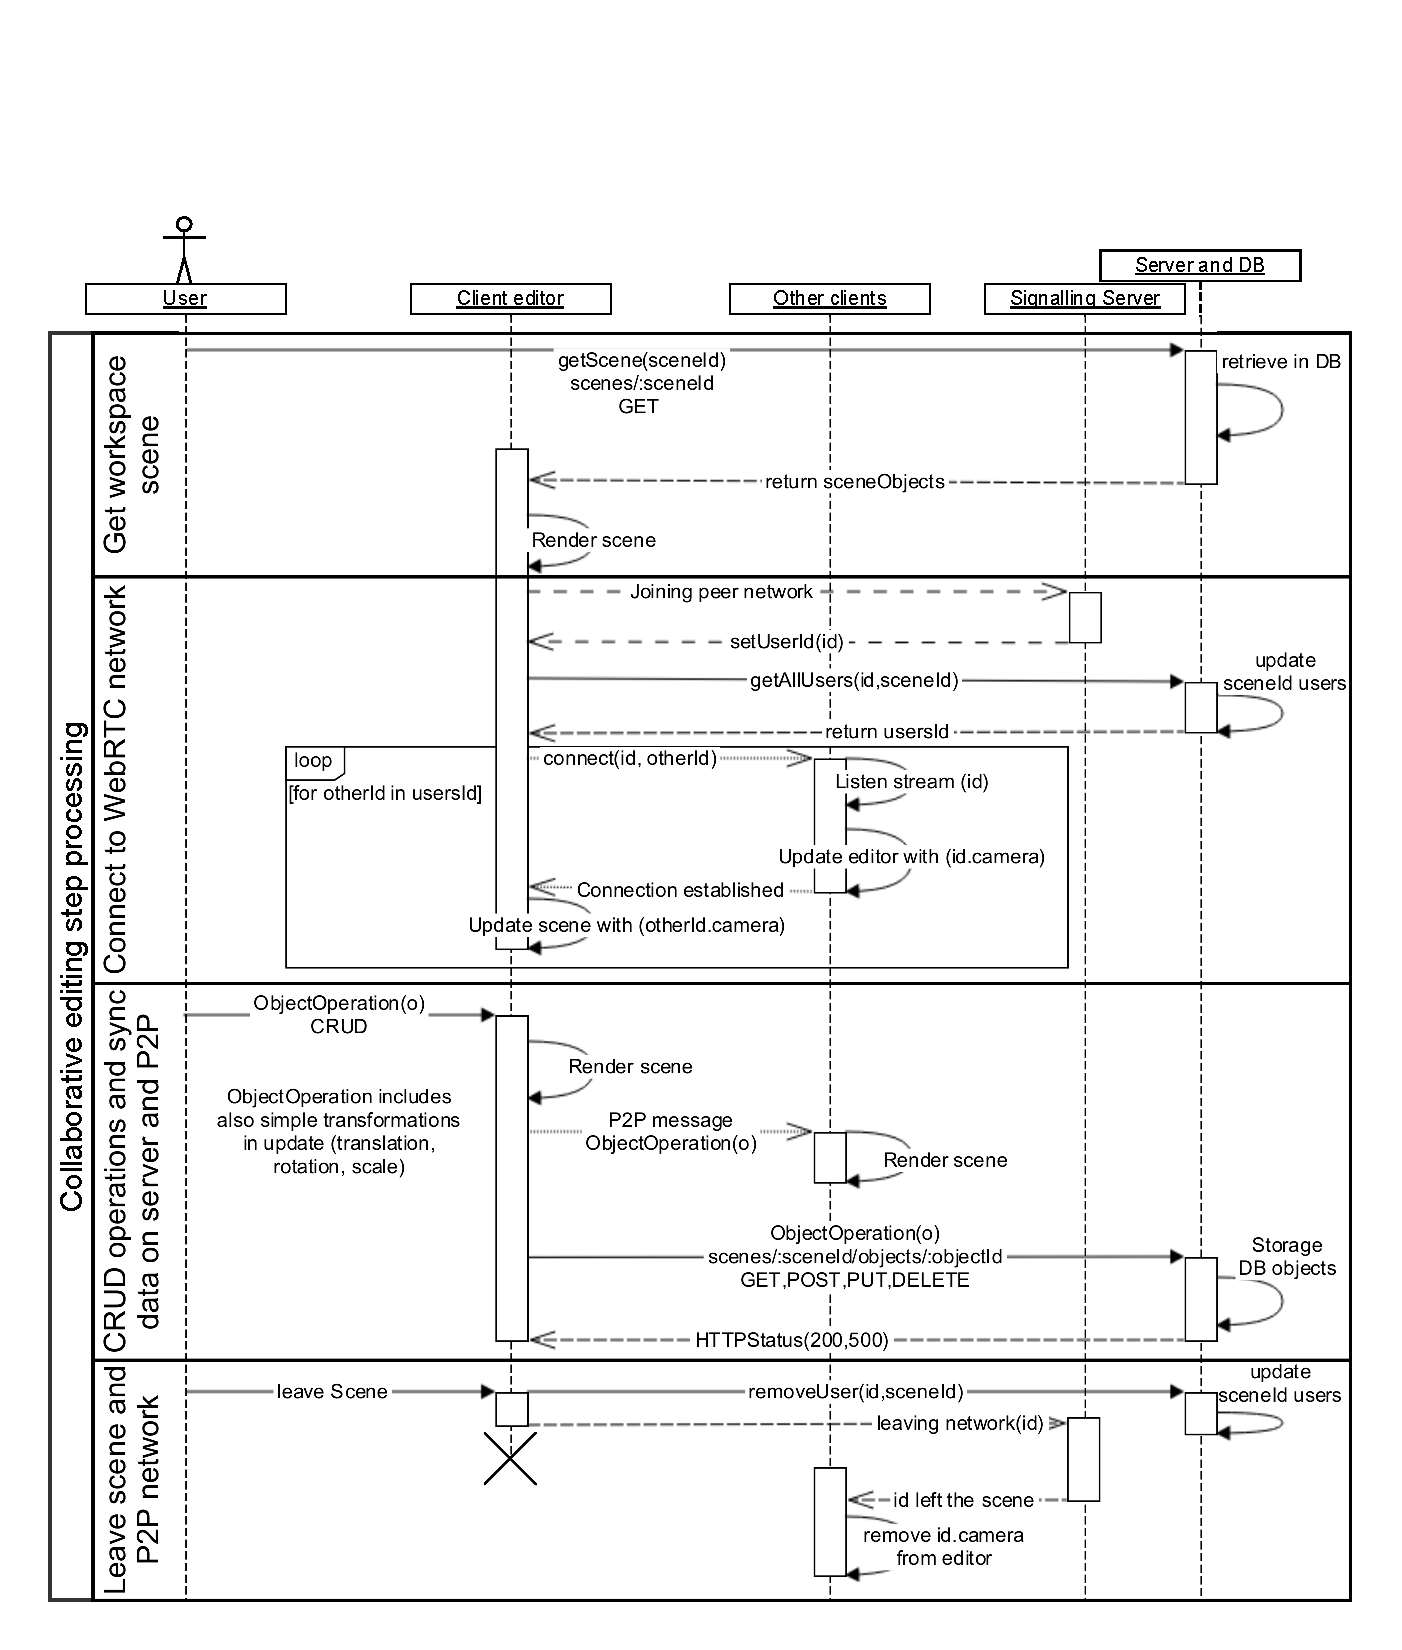
\includegraphics[trim={0 0 0 3cm},clip,width=1\columnwidth]
	{eps/sequence_wscg.eps}
	\caption{Diagramme de séquence de la gestion de la session dans une 
	architecture \og orientée état\fg{}}
	\label{fig:sequence_state}
\end{figure}

%
%We propose to auto connect users on a scene with a We- bRTC connection. As 
%each user send their ID to the database at their arrival, they also retrieve those 
%which where already present on the scene. We are able to cre- ate a full mesh 
%topology network in order to make them communicate the updates.
%
%Even if we have a full mesh topology, the P2P message layer is more similar 
%the 
%star topology. Indeed, the Fig- ure 2 shows the path of a sent message 
%operation 
%on the connection and it is only sent to the one degree neigh- bors of the original 
%broadcaster (the “B” node on the Figure 2).
%
%
%We choose to keep reliable and in order delivery for now. The RTCDataChannel 
%API supports many data types (strings, binary types: Blob, ArrayBuffer. . . ). 
%These types are helpful in a 3D multi user environment to broadcast messages 
%including the objets and their transformations. We tried to limit the amount of 
%data 
%by sending only relevant information but there is actually no particular 
%optimization. The channel can be over- feed when an object is imported then 
%pushed through the network.
%

\subsubsection{Gestion de la synchronisation et de la cohérence}
\label{sec:synchronisation-client-serveur}

Les travaux \cite{Desprat2015a} et \cite{Desprat2015b} présentent une version 
naïve du processus de synchronisation. La cohérence est garantie par un système 
de verrouillage des objets. Cela évite notamment les sélections concurrente et par 
conséquent les éditions concurrentes. 
Lors de la récupération de la scène, elle est considérée comme cohérente. 
Ensuite, le choix d'avoir des connexions \gls{P2P} ordonnées et fiables ainsi qu'un 
maillage de pair complet, implique que toute donnée envoyée par un pair est 
forcément reçue par les autres. 

Lors de la connexion d'un nouveau client a lieu la synchronisation des deux 
systèmes de persistance pour obtenir les mises à jour : 
\improve{l'échange des mises à jour entre le client (persistance à court terme) et la 
	base de données (à long terme) afin de synchroniser les deux éléments avec. 
	La base de données peut également servir en cas de conflit important ; elle sert 
	de référent.}
\begin{enumerate}
	\item depuis le client, où l'on distingue trois cas :
	\begin{enumerate}
		\item travail "\textit{offline}" (hors ligne) : l'utilisateur a travaillé hors ligne et 
		doit maintenant publier "en ligne" son travail. Les mises à jour publiées sur la 
		base de données ; le serveur vérifie si aucun conflit ne survient puis 
		fusionne (\textit{merge}) les nouvelles entrées avec l'existant; 
		
		\item travail "\textit{serverless}" (en collaboration avec d'autres pairs sans le 
		serveur) : dans le cas où le serveur est absent, les clients peuvent continuer 
		de créer en collaborant. Ces données n'étant stockées que sur le client, il est 
		nécessaire de les transmettre à la base de données dès qu'une connexion 
		est possible. 
		Cela peut être fait en une fois ou de manière partagée\improve{ça veut dire 
			quoi?};
		
		\item travail "\textit{online}" (en collaboration avec d'autres pairs avec le 
		serveur) : le client envoie régulièrement \improve{combien de temps} ses 
		nouvelles modifications pour qu'elles soient intégrées à la base de données.
	\end{enumerate}
	\item depuis la base de données :
	Le client reçoit toutes les nouvelles mises à jour de la scène depuis la dernière 
	fois qu'il s'est connecté. Cela peut également inclure des mises à jour qui sont 
	en conflit avec ce qu'il y a dans son propre espace de stockage qu'il lui faut 
	donc modifier.
	Dans le cas où un utilisateur est seul connecté, la base de données est la 
	seule source disponible pour la mise à jour du client. 
\end{enumerate}


Le fait de synchroniser un client avec une base de données NoSQL dès que cela 
est possible permet de supporter les connexions intermittentes comme pour les 
appareils mobiles dans cette architecture ; cette approche est connue sans le nom 
de \og\textit{ offline first}\fg{} \cite{Gadea2016}.
\subsubsection{Topologie et protocole d'échange}
Cette architecture est basée sur une topologie de maillage complet (\textit{full 
mesh topology}) pour le réseau \gls{P2P}.
Les échanges se font donc à deux niveaux: entre les pairs ainsi qu'entre chaque 
pair et la base de données. Pour le premier niveau, la couche réseau \gls{P2P} est 
assez 
naïve dans le sens où les connexions sont considérées comme fiables et 
ordonnées, le client n'a alors qu'à publier toutes les modifications qu'il effectue et 
les envoyer à tous les clients (auxquels il est nécessairement connecté).
Les pairs échange des différentiels d'état sur les objets. Ces messages ne 
contiennent pas d'information sémantique sur le type d'action effectuée par chaque 
utilisateur. 

\subsubsection{Discussion des problématiques liées à une architecture de 
communication orientrée \og états\fg{}}

La base de données centralisée est beaucoup sollicitée lors des sessions 
collaboratives, ce qui peut mener à une surcharge similaire aux architectures 
uniquement client serveur. 
En combinant client-serveur et \gls{P2P}, la charge aurait dû être réduite et 
transférée aux autres pairs, notamment lors de la phase de récupération d'une 
nouvelle scène qui repose entièrement sur le serveur. 
Chaque pair assume la responsabilité dans l'envoi de ses modifications à tous les 
autres pairs. Cette tâche ne profite pas du réseau \gls{P2P} de manière optimale 
car la topologie ne profite pas de la fonction relai des pairs. Cela pourrait alléger  la 
distribution dans la couche \gls{P2P} et responsabiliser un peu plus les pairs pour 
faciliter le passage à l'échelle.
En effet, la topologie en maillage complet limite le passage à l'échelle car le 
nombre de connexion va croitre de manière exponentielle. 

Par ailleurs, les requêtes \gls{CRUD} ne sont pas très expressives concernant le 
métier. 
Aucune vérification n'est donc effectuée sur la validité des données transmises 
dans cette architecture. De plus, il peut arriver, du fait de latences réseaux que les 
modifications des différents utilisateurs s'entrelacent à l'arrivée et ne rendent pas 
l'intention de l'utilisateur. Cela peut mener à des dé-synchronisations fortes.

Concernant la gestion de la concurrence, l'utilisation d'une solution pessimiste 
dans un environnement \gls{P2P} peut parfois mener à des inter-blocages si un 
utilisateur quitte la scène sans avoir relâché l'objet, c'est à dire, sans en avoir 
informé la base de données et les autres 
utilisateurs. 
Même si l'application peut prendre le relais, et permettre la relache du 
verrou au bout d'un certain temps, l'expérience utilisateur peut être dégradée 
pendant cette période.
Le maintient de la cohérence est a peu près garanti dans ce modèle si l'on 
considère un environnement où la fréquence des modifications n'est pas très 
élevée, que tous les clients communique leur horloge local pour établir un 
référentiel de temps concernant les mises à jour. 

Enfin, le transfert par différentiel d'état utilisé pour réduire la taille des 
données liées au changement d'état des objets lors de la transmission des 
données peut varier grandement selon le type de changement 
effectué, rendant peu prédictibilité la charge des canaux de communication. 
%
%Some issues remain in RTCDataChannel API : the com- patibility and 
%interoperability is still not complete be- tween browsers6, some browsers (like 
%Chrome) im- pose a send limit (about 6MB) for the data transmitting through 
%DataConnections and the security of the com- munication is still vulnerable7. 
%The 
%system overview (Figure 4) illustrates the communication architecture topology 
%between the peer clients and server (plus sig- naling).
